% questions.tex —— 2015 年·上海卷·文科 · 题目内容片段（无答案）
% 由 tools/generate_projects.py 依来源总账自 2015/2015_数学真题_上海文_试题.md 生成，勿手改（改源 MD 后重跑）


\gkpart{数学}

\begin{gktip}
\textbf{来源说明}：本题面依据固定源 PDF 全 2 页逐题核对（p1＝页 979：左栏填空 1–14、中栏选择 15–18 与解答 19、右栏解答 20；p2＝页 980：左栏解答 21、中栏解答 22、右栏解答 23）。原卷为 \textbf{A3 横向（1190.55 × 841.89 pt）三栏书刊合排}——栏位实测：左栏 42.69–404.18、中栏 414.85–776.35、右栏 787.02–1148.52 pt（栏宽 361.50、中缝 10.67 pt），阅读序＝左→中→右；\textbf{页脚仅印合订本书页页码 979／980}（位于页面底部正中，非卷内页码），\textbf{无页眉}。标题「2015 普通高等学校招生考试（上海卷文）」为通栏排印。\textbf{全卷不印分值、不印题量、不印「考生注意」栏}——三处节头逐字仅「一、填空题」「二、选择题」「三、解答题」四字，解答题无「（本题满分 N 分）」行（全段「分」字仅 1 处、为第 22 题「分别」之「分」）；总分 150 为结构推断，\textbf{卷面无凭据}，本文件不作补写。

\textbf{源制作体系判定（\texttt{pdffonts}／\texttt{pdftotext -layout}／\texttt{pdfimages -list} 实测）}：源\textbf{不是扫描件，而是 LaTeX（Computer Modern 系）重排产物}——\texttt{pdfimages -list} 零命中（全页无任何位图），\texttt{pdftocairo -svg} 第 1 页 353 条矢量路径／0 个 \texttt{<image>}；嵌入字体 \textbf{16 个}：中文 \textbf{STSong（宋体正文）／STHeiti（黑体标题与节头）}，拉丁与数学 \textbf{LMRoman10／LMRoman12-Bold／CMR10／CMR7／CMR5／CMMI10／CMMI7／CMSY10／CMSY7／CMEX10／MSAM10／CMMIB10}，及中文数学延展件 \textbf{Yhcmex（yhmath，弧记号）}。\textbf{文本层完整可读}（无私用区 PUA、无提取丢失）——本文件以页面图像为准录入、以文本层与逐字字体表交叉校验。故本卷的「源内异常」均为\textbf{矢量坐标或排版瑕疵}，不存在扫描噪声类问题。

\textbf{标点与字样约定（实测）}：① \textbf{题号与句末}源内为半角 \texttt{.}，按全库约定写作全角「．」；② \textbf{正文句读}源内为半角 ASCII 逗号而顿号「、」为全角 CJK——本文件按全库约定把句中逗号归一为全角「，」，\textbf{顿号照源保留}（源内「男、女教师」等处的顿号即全角「、」），内容零改动；③ \textbf{选择题选项标号}源内为\textbf{半角「(A)」}，按本库「选项照源」纪律\textbf{照录为 \texttt{(A)}}；④ \textbf{作答空}：填空题为统一长度横线（实测全 14 题均 31.49 pt，写作 \texttt{\gkblank{}}），选择题为右对齐空括号（写作「（　）」）；⑤ \textbf{正文层括号}（如源内半角的「(结果用数值表示)」）\textbf{按全库约定归一为全角「（）」}；\textbf{数学模式内部的括号照源保持半角}（如 \((p>0)\)、\((m\geqslant 2,\ m\in\mathbf{N}^{*})\) 均在数学定界内）；⑥ \textbf{不等号}源为 MSAM10 的水平横杠形（U+2A7D／U+2A7E），写 \(\leqslant\)／\(\geqslant\)；⑦ \textbf{实数集／正整数集／复数集}源为粗正体，写 \(\mathbf{R}\)／\(\mathbf{N}^{*}\)／\(\mathbf{C}\)；⑧ \textbf{虚数单位}源为正体，写 \(\mathrm{i}\)；⑨ \textbf{向量}源为 CMMIB10 粗斜体、\textbf{无箭头}（矢量笔画清单无箭头笔画），写 \(\boldsymbol{a}\) 形式；⑩ 行内分式一律排作显示风格（如 \(\dfrac{a}{b}\)，与源内堆叠分式同形）；⑪ \textbf{弧记号}源为 Yhcmex 宽弧重音，写 \(\overset{\frown}{AB}\)（本库 preamble 未载 yhmath，全库先例一致）。

\textbf{存疑与登记}（源内异常一律照录；完整清单见工作档 \texttt{page-map.md} §7 A1–A19）：① 第 14 题「\(6\pi\)\textbf{．}且」以句点代逗号（1200 dpi 确认：基线实心方针点、LMRoman10；上下文为并列条件从句）——\textbf{照录保留句点、不径改}；② 第 5 题用顿号连接增广矩阵与「解为」、方程组花括号后\textbf{直接接「则」无标点}、组末行带尾逗号（\texttt{y=5,}）——三处悉数照录；③ 第 19 题图\textbf{源内瑕疵两处}（照源复刻）：图内 \(C\) 位于椭圆参数角 249.30°——题设「半圆弧 \(AB\) 的中点」应为 270.000°，\textbf{偏 20.70°}；母线 \(PA\)、\(PB\) 照源画作椭圆\textbf{切线}，落点比标注点 \(A\)、\(B\) 高 4.847 pt、各内收 1.193 pt（同图 \(E\) 则严格为弧 \(CB\) 中点、与题设一致）；④ 第 21 题图为\textbf{精确作图}（直角 90.000000°、三边按 1 千米 = 1 厘米精确）；⑤ 第 19 题题干两处弧记号源内为 Yhcmex 相邻两档宽弧（墨迹宽 14.46／16.62 pt），文本层 ToUnicode 分别落为 U+02DC／U+00AF——系映射落点差异，转写统一为 \(\overset{\frown}{}\) 不作区分。

\textbf{题图}：共 2 处——第 19 题\textbf{圆锥}（顶点 \(P\)、底面圆心 \(O\)、直径 \(AB\)、\(C\) 为半圆弧 \(\overset{\frown}{AB}\) 中点、\(E\) 为劣弧 \(\overset{\frown}{CB}\) 中点；椭圆底，远侧半弧与 \(PO\)、\(AB\)、\(AC\)、\(OC\)、\(OE\) 为虚线）与第 21 题\textbf{直角路线图}（\(O\)、\(P\)、\(Q\) 三点，直角在 \(P\)）。两图均为矢量绘制，逐要素实测见工作档 \texttt{figure-inventory.md}。
\end{gktip}

\gkpart{试题}

\gkpart{一、填空题}

\begin{question}
\gkti{1}函数 \(f(x)=1-3\sin^{2}x\) 的最小正周期为\gkblank{}．

\end{question}
\begin{question}
\gkti{2}设全集 \(U=\mathbf{R}\)．若集合 \(A=\{1,2,3,4\}\)，\(B=\{x\mid 2\leqslant x\leqslant 3\}\)，则 \(A\cap\complement_{U}B=\)\gkblank{}．

\end{question}
\begin{question}
\gkti{3}若复数 \(z\) 满足 \(3z+\overline{z}=1+\mathrm{i}\)，其中 \(\mathrm{i}\) 为虚数单位，则 \(z=\)\gkblank{}．

\end{question}
\begin{question}
\gkti{4}设 \(f^{-1}(x)\) 为 \(f(x)=\dfrac{x}{2x+1}\) 的反函数，则 \(f^{-1}(2)=\)\gkblank{}．

\end{question}
\begin{question}
\gkti{5}若线性方程组的增广矩阵为 $\begin{pmatrix} 2 & 3 & c_{1}\\ 0 & 1 & c_{2} \end{pmatrix}$、解为 $\begin{cases} x=3,\\ y=5, \end{cases}$ 则 \(c_{1}-c_{2}=\)\gkblank{}．

\end{question}
\begin{question}
\gkti{6}若正三棱柱的所有棱长均为 \(a\)，且其体积为 \(16\sqrt{3}\)，则 \(a=\)\gkblank{}．

\end{question}
\begin{question}
\gkti{7}抛物线 \(y^{2}=2px\ (p>0)\) 上的动点 \(Q\) 到焦点的距离的最小值为 1，则 \(p=\)\gkblank{}．

\end{question}
\begin{question}
\gkti{8}方程 \(\log_{2}(9^{x-1}-5)=\log_{2}(3^{x-1}-2)+2\) 的解为\gkblank{}．

\end{question}
\begin{question}
\gkti{9}若 \(x\)，\(y\) 满足 $\begin{cases} x-y\geqslant 0,\\ x+y\leqslant 2,\\ y\geqslant 0, \end{cases}$ 则目标函数 \(f=x+2y\) 的最大值为\gkblank{}．

\end{question}
\begin{question}
\gkti{10}在报名的 3 名男教师和 6 名女教师中，选取 5 人参加义务献血，要求男、女教师都有，则不同的选取方式的种数为\gkblank{}．（结果用数值表示）

\end{question}
\begin{question}
\gkti{11}在 \(\left(2x+\dfrac{1}{x^{2}}\right)^{6}\) 的二项展开式中，常数项等于\gkblank{}．（结果用数值表示）

\end{question}
\begin{question}
\gkti{12}已知双曲线 \(C_{1}\)，\(C_{2}\) 的顶点重合，\(C_{1}\) 的方程为 \(\dfrac{x^{2}}{4}-y^{2}=1\)，若 \(C_{2}\) 的一条渐近线的斜率是 \(C_{1}\) 的一条渐近线的斜率的 2 倍，则 \(C_{2}\) 的方程为\gkblank{}．

\end{question}
\begin{question}
\gkti{13}已知平面向量 \(\boldsymbol{a}\)，\(\boldsymbol{b}\)，\(\boldsymbol{c}\) 满足 \(\boldsymbol{a}\perp\boldsymbol{b}\)，且 \(\{|\boldsymbol{a}|,|\boldsymbol{b}|,|\boldsymbol{c}|\}=\{1,2,3\}\)，则 \(|\boldsymbol{a}+\boldsymbol{b}+\boldsymbol{c}|\) 的最大值是\gkblank{}．

\end{question}
\begin{question}
\gkti{14}已知函数 \(f(x)=\sin x\)．若存在 \(x_{1}\)，\(x_{2}\)，\(\cdots\)，\(x_{m}\) 满足 \(0\leqslant x_{1}<x_{2}<\cdots<x_{m}\leqslant 6\pi\)．且 \(|f(x_{1})-f(x_{2})|+|f(x_{2})-f(x_{3})|+\cdots+|f(x_{m-1})-f(x_{m})|=12\ (m\geqslant 2,\ m\in\mathbf{N}^{*})\)，则 \(m\) 的最小值为\gkblank{}．

\end{question}
\gkpart{二、选择题}

\begin{question}
\gkti{15}设 \(z_{1}\)，\(z_{2}\in\mathbf{C}\)，则“\(z_{1}\)，\(z_{2}\) 均为实数”是“\(z_{1}-z_{2}\) 是实数”的（　）

(A) 充分非必要条件　　(B) 必要非充分条件

(C) 充要条件　　(D) 既非充分又非必要条件

\end{question}
\begin{question}
\gkti{16}下列不等式中，与不等式 \(\dfrac{x+8}{x^{2}+2x+3}<2\) 解集相同的是（　）

(A) \((x+8)(x^{2}+2x+3)<2\)　　(B) \(x+8<2(x^{2}+2x+3)\)

(C) \(\dfrac{1}{x^{2}+2x+3}<\dfrac{2}{x+8}\)　　(D) \(\dfrac{x^{2}+2x+3}{x+8}>\dfrac{1}{2}\)

\end{question}
\begin{question}
\gkti{17}已知点 \(A\) 的坐标为 \((4\sqrt{3},1)\)，将 \(OA\) 绕坐标原点 \(O\) 逆时针旋转 \(\dfrac{\pi}{3}\) 至 \(OB\)，则点 \(B\) 的纵坐标为（　）

(A) \(\dfrac{3\sqrt{3}}{2}\)　(B) \(\dfrac{5\sqrt{3}}{2}\)　(C) \(\dfrac{11}{2}\)　(D) \(\dfrac{13}{2}\)

\end{question}
\begin{question}
\gkti{18}设 \(P_{n}(x_{n},y_{n})\) 是直线 \(2x-y=\dfrac{n}{n+1}\ (n\in\mathbf{N}^{*})\) 与圆 \(x^{2}+y^{2}=2\) 在第一象限的交点，则极限 \(\lim\limits_{n\to\infty}\dfrac{y_{n}-1}{x_{n}-1}=\)（　）

(A) \(-1\)　(B) \(-\dfrac{1}{2}\)　(C) \(1\)　(D) \(2\)

\end{question}
\gkpart{三、解答题}

\Needspace{0.4\textheight}
\begin{question}
\gkti{19}如图，圆锥的顶点为 \(P\)，底面圆心为 \(O\)，底面的一条直径为 \(AB\)，\(C\) 为半圆弧 \(\overset{\frown}{AB}\) 的中点，\(E\) 为劣弧 \(\overset{\frown}{CB}\) 的中点，已知 \(PO=2\)，\(OA=1\)，求三棱锥 \(P-AOC\) 的体积，并求异面直线 \(PA\) 与 \(OE\) 所成角的余弦值．
\nopagebreak[4]
\begin{center}% 第 19 题圆锥图：按固定源内容流矢量层精确值复刻（1 pt → 0.03515 cm）。
% 原点取底面圆心 O（源页 (693.454, 395.647) pt），y 向上。
% 底面为透视缩扁的椭圆：半长轴 68.0346、半短轴 25.7095（PO/OA = 2.00000 与题设严格一致）。
% 实线 4 条：母线 PC、母线 PA/PB（照源画作椭圆切线，落点 (±66.842, +4.847) 不在 A/B 上）、
% 近侧半弧（下，参数角 170°→350°）；虚线 6 条：轴线 PO、直径 AB、弦 AC、
% 半径 OC 与 OE、远侧半弧（上，参数角 10°→170°）。虚线节距照源 [on 2.989 off 2.989]。
% 源内瑕疵照录：C 位于参数角 249.30°（题设「半圆弧 AB 的中点」应为 270.000°、偏 20.70°）；
% E 严格为弧 C→B 中点（304.63°，与题设一致）；母线端点比 A/B 高 4.847 pt、各内收 1.193 pt。
% 全图无点记号、无箭头、无填充；六个标签照源文本原点（基线左端）定位。
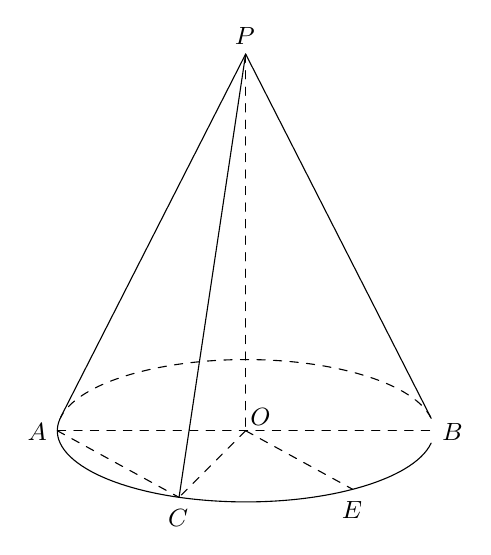
\begin{tikzpicture}[line cap=round,line join=round,font=\small,x=0.03515cm,y=0.03515cm]
% ===== 椭圆底（两半弧照源分开绘制：远侧虚线 / 近侧实线）=====
\draw[dash pattern=on 2.989pt off 2.989pt, line width=0.398bp] (67.0001,4.4643) arc [start angle=10, end angle=170, x radius=68.0346, y radius=25.7095];   % 远侧半弧（上，虚线）
\draw[line width=0.398bp] (-66.9989,4.4643) arc [start angle=170, end angle=350, x radius=68.0346, y radius=25.7095];   % 近侧半弧（下，实线）
% ===== 实线 3 条（母线；PA/PB 照源为切线画法）=====
\draw[line width=0.398bp] (0,136.069)--(-24.067,-24.0669);   % P–C
\draw[line width=0.398bp] (0,136.069)--(-66.842,4.8471);   % P–左切点（PA）
\draw[line width=0.398bp] (0,136.069)--(66.842,4.8471);   % P–右切点（PB）
% ===== 虚线 5 条（轴线/底面辅助线）=====
\draw[dash pattern=on 2.989pt off 2.989pt, line width=0.398bp] (0,136.069)--(0,0);   % P–O（轴线）
\draw[dash pattern=on 2.989pt off 2.989pt, line width=0.398bp] (-68.0346,0)--(68.0344,0);   % A–B（直径）
\draw[dash pattern=on 2.989pt off 2.989pt, line width=0.398bp] (-68.0346,0)--(-24.067,-24.0669);   % A–C（弦）
\draw[dash pattern=on 2.989pt off 2.989pt, line width=0.398bp] (0,0)--(-24.067,-24.0669);   % O–C（半径）
\draw[dash pattern=on 2.989pt off 2.989pt, line width=0.398bp] (0,0)--(38.695,-21.176);   % O–E（半径）
% ===== 标注（照源文本原点＝基线左端，显式坐标）=====
\node[anchor=base west,inner sep=0] at (-4.1,139.456) {\(P\)};
\node[anchor=base west,inner sep=0] at (1.485,2.048) {\(O\)};
\node[anchor=base west,inner sep=0] at (-78.946,-3.588) {\(A\)};
\node[anchor=base west,inner sep=0] at (70.763,-3.588) {\(B\)};
\node[anchor=base west,inner sep=0] at (-28.195,-34.629) {\(C\)};
\node[anchor=base west,inner sep=0] at (34.516,-31.737) {\(E\)};
\end{tikzpicture}
\end{center}
\nopagebreak[4]
\end{question}
\begin{question}
\gkti{20}已知函数 \(f(x)=ax^{2}+\dfrac{1}{x}\)，其中 \(a\) 为常数．

（1） 根据 \(a\) 的不同取值，判断函数 \(f(x)\) 的奇偶性，并说明理由；

（2） 若 \(a\in(1,3)\)，判断函数 \(f(x)\) 在 \([1,2]\) 上的单调性，并说明理由．

\Needspace{0.4\textheight}
\end{question}
\begin{question}
\gkti{21}如图，\(O\)，\(P\)，\(Q\) 三地有直道相通，\(OP=3\) 千米，\(PQ=4\) 千米，\(OQ=5\) 千米．现甲、乙两警员同时从 \(O\) 地出发匀速前往 \(Q\) 地，经过 \(t\) 小时，他们之间的距离为 \(f(t)\)（单位：千米）．甲的路线是 \(OQ\)，速度为 5 千米/小时，乙的路线是 \(OPQ\)，速度为 8 千米/小时．乙到达 \(Q\) 地后在原地等待．设 \(t=t_{1}\) 时，乙到达 \(P\) 地；\(t=t_{2}\) 时，乙到达 \(Q\) 地．

（1） 求 \(t_{1}\) 与 \(f(t_{1})\) 的值；

（2） 已知警员的对讲机的有效通话距离是 3 千米．当 \(t_{1}\leqslant t\leqslant t_{2}\) 时，求 \(f(t)\) 的表达式，并判断 \(f(t)\) 在 \([t_{1},t_{2}]\) 上的最大值是否超过 3？说明理由．
\nopagebreak[4]
\begin{center}% 第 21 题直角路线图：按固定源内容流矢量层精确值复刻（1 pt → 0.03515 cm）。
% 原点取顶点 O（源页 (306.812, 523.641) pt），y 向上。
% 三边 O–P（水平）、P–Q（竖直）、Q–O（斜边），直角精确在 P（90.000000°）；
% 三边按 1 千米 = 1 厘米精确作图（比例尺 28.3468 pt/km，本库少见之满分构图）。
% 无直角记号、无顶点圆点、无长度/角度标注、无箭头、无填充；三个标签照源文本原点定位。
\begin{tikzpicture}[line cap=round,line join=round,font=\small,x=0.03515cm,y=0.03515cm]
% ===== 三条边（均实线）=====
\draw[line width=0.398bp] (0,0)--(85.04,0);   % O–P
\draw[line width=0.398bp] (85.04,0)--(85.04,113.387);   % P–Q
\draw[line width=0.398bp] (85.04,113.387)--(0,0);   % Q–O
% ===== 标注（照源文本原点＝基线左端，显式坐标）=====
\node[anchor=base west,inner sep=0] at (-9.082,-8.519) {\(O\)};
\node[anchor=base west,inner sep=0] at (85.872,-8.519) {\(P\)};
\node[anchor=base west,inner sep=0] at (80.89,117.794) {\(Q\)};
\end{tikzpicture}
\end{center}
\nopagebreak[4]
\end{question}
\begin{question}
\gkti{22}已知椭圆 \(x^{2}+2y^{2}=1\)，过原点的两条直线 \(l_{1}\) 和 \(l_{2}\) 分别与椭圆交于点 \(A\)，\(B\) 和 \(C\)，\(D\)．记 \(\triangle AOC\) 的面积为 \(S\)．

（1） 设 \(A(x_{1},y_{1})\)，\(C(x_{2},y_{2})\)．用 \(A\)，\(C\) 的坐标表示点 \(C\) 到直线 \(l_{1}\) 的距离，并证明 \(S=\dfrac{1}{2}|x_{1}y_{2}-x_{2}y_{1}|\)；

（2） 设 \(l_{1}:y=kx\)，\(C\left(\dfrac{\sqrt{3}}{3},\dfrac{\sqrt{3}}{3}\right)\)，\(S=\dfrac{1}{3}\)，求 \(k\) 的值．

（3） 设 \(l_{1}\) 与 \(l_{2}\) 的斜率之积为 \(m\)，求 \(m\) 的值，使得无论 \(l_{1}\) 与 \(l_{2}\) 如何变动，面积 \(S\) 保持不变．

\end{question}
\begin{question}
\gkti{23}已知数列 \(\{a_{n}\}\) 与 \(\{b_{n}\}\) 满足 \(a_{n+1}-a_{n}=2(b_{n+1}-b_{n})\)，\(n\in\mathbf{N}^{*}\)．

（1） 若 \(b_{n}=3n+5\)，且 \(a_{1}=1\)，求 \(\{a_{n}\}\) 的通项公式；

（2） 设 \(\{a_{n}\}\) 的第 \(n_{0}\) 项是最大项，即 \(a_{n_{0}}\geqslant a_{n}\)（\(n\in\mathbf{N}^{*}\)），求证：\(\{b_{n}\}\) 的第 \(n_{0}\) 项是最大项；

（3） 设 \(a_{1}=3\lambda<0\)，\(b_{n}=\lambda^{n}\)（\(n\in\mathbf{N}^{*}\)），求 \(\lambda\) 的取值范围，使得对任意 \(m\)，\(n\in\mathbf{N}^{*}\)，\(a_{n}\neq0\)，且 \(\dfrac{a_{m}}{a_{n}}\in\left(\dfrac{1}{6},6\right)\)．

\end{question}